\section{Datenmanagement}
In diesem Kapitel wird der Use-Case vorgestellt. Anschliessend wird die für die  Abwicklung des Use-Case benötigte Datenarchitektur beschrieben. Die ausgewählte Datenbank Technologie, sowie die Projektarchitektur sind in den letzten zwei Unterkapiteln ersichtlich.


\subsection{Use-Case}
\label{subsec: use case}

Das Projektteam hat sich dazu entschieden, Daten von Filmen zu analysieren, um den folgenden Use-Case zu bearbeiten:
\\
Ein Investor möchte einen neuen Blockbuster im Genre der Action-Filme in die Kinos bringen. Das Zielpublikum sind alle Personen, die zwischen 18 und 30 Jahre alt sind. Ziel des Investors ist ein möglichst erfolgreicher Film in einer bestimmten Kultur\footnote{Beispielsweise Hollywood hat als Produktionsland (zukünftig als Land abgekürzt) die USA, Bollywood hat Indien.}. Um dies zu erreichen, ist er auf der Suche nach dem perfekten Filmteam. Dieses Team soll sich aus folgenden Rollen zusammensetzen:
\begin{itemize}
	\item ein Produzent
	\item ein Drehbuchautor
	\item ein Regisseur
	\item drei Schauspieler
	\item drei Schauspielerinnen
\end{itemize}

Daraus ergibt sich folgende Entscheidungsfrage:\\
\begin{tcolorbox}
    Welches Filmteam soll angeheuert werden, um den grösstmöglichen Erfolg beim genannten Zielpublikum zu erreichen?
\end{tcolorbox}

Für die Beantwortung der Use-Case Entscheidungsfrage muss die Komplexität der Realität reduziert werden. Dies wird über Annahmen und Vereinfachungen erreicht. Beispielsweise werden die jeweiligen Filmrollen isoliert betrachtet. Für ein objektives Bewerten der erbrachten Leistung einer Person müssen Bewertungskriterien eingeführt werden. Mit einem oder wenigen Performance Parametern können schliesslich die einzelnen Personen in ihren Rollen miteinander verglichen und bewertet werden.


\subsection{Datenarchitektur}
Eine geeignete Datenstruktur ist notwendig für das erfolgreiche Auswerten des Use-Cases. \autoref{fig:Datenarchitekur} zeigt die notwendige Datenstruktur mit den entsprechenden Attributen. 

\begin{figure}[H]
	\centering
	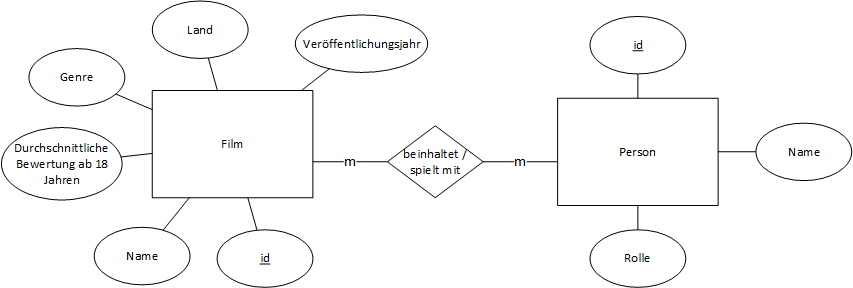
\includegraphics[width=1.0\columnwidth]{2_Datenmanagement/Bilder/Datenarchitektur.png}
	\caption{Datenarchitektur des Use-Cases.}
	\label{fig:Datenarchitekur}
\end{figure}

\subsection{Datenbanktechnologie}

Für diese Anwendung wird eine \textit{MySQL} Datenbanktechnologie verwendet. Folgende Argumente sprechen für die Wahl von \textit{MySQL}:
\begin{itemize}
	\item Weit verbreitete Technologie~\cite{db-engines.com} mit umfangreicher Community.
	\item Das Volumen der Datenbasis ist in der Megabyte-Grössenordnung. Dementsprechend eignet sich ein bewährtes relationales Datenbanksystem.
	\item Das Arbeiten mit Metadaten in Tabellen bietet sich für die Datenbasis an. Die Vorteile von No-SQL Datenbanksystemen sind beim gegebenen Datensatz unbedeutend.
\end{itemize}

\subsection{Projektarchitektur}
Um die nachfolgenden Beschreibungen sowie Erläuterungen besser zu verstehen, wird in diesem Unterkapitel die gesamte Architektur des Projekts dargestellt. Die \autoref{fig:Projektarchitektur} zeigt diese Architektur unterteilt in mehreren Schichten. Die eigentlichen Datenbank-Operationen finden auf der Daten-Schicht statt. Die Aufbereitung der Abfragen wird in der Schicht der Business-Logik durchgeführt. Schliesslich werden in der Präsentations-Schicht die Resultate als auch die Abfragemöglichkeiten über einen Webserver auf einer Webseite dargestellt.

\begin{figure}[H]
	\centering
	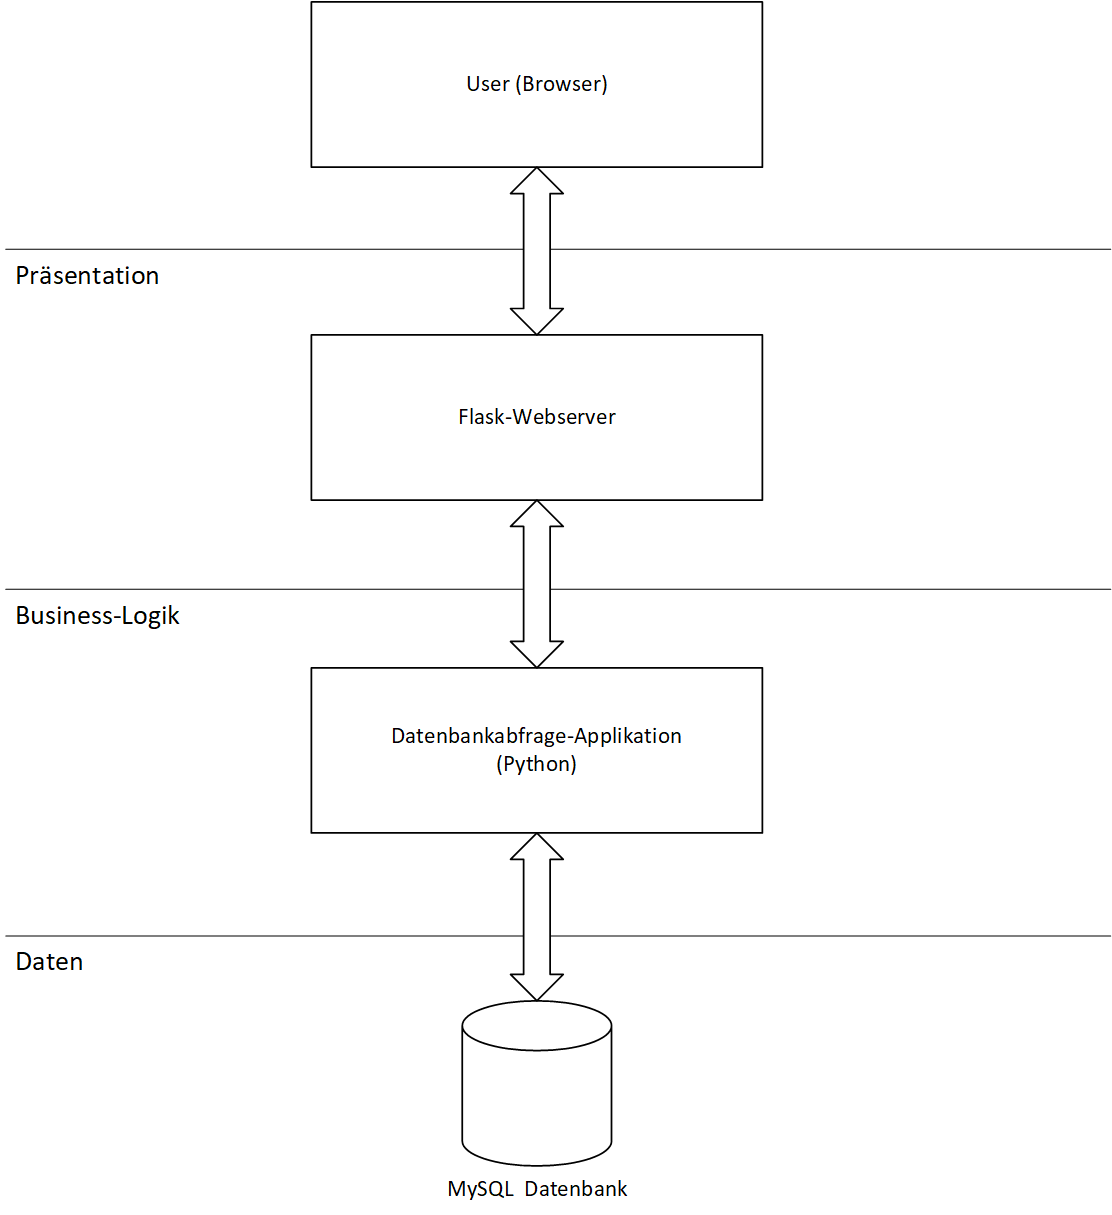
\includegraphics[width=0.9\columnwidth]{2_Datenmanagement/Bilder/ProjektArchitektur.png}
	\caption{Projektarchitektur unterteilt in Schichten.}
	\label{fig:Projektarchitektur}
\end{figure}